\documentclass{article}

\usepackage{geometry}
\usepackage{afterpage}
\usepackage{graphicx}
\usepackage{outlines}
\usepackage{hyperref}
\usepackage{changepage}
\usepackage{amssymb}
\usepackage{amsfonts}
\usepackage{pdflscape}
\usepackage{amsmath}
\usepackage{amsthm}
\usepackage{blindtext}

\author{Astrid Augusta Yu}
\title{CSC 348 -- Midterm}
\date{\today}

\newcommand{\contradiction}{$\rightarrow\leftarrow$}
\newtheorem{theorem}{Theorem}
\newtheorem{lemma}{Lemma}
\newtheorem{claim}{Claim}

\begin{document}
\maketitle
\tableofcontents

\section{Questions}
\begin{outline}[enumerate]
    \1 $P = \text{``I can assign partial credit for a question''}$

        $Q = \text{``You leave it blank''}$

        $(\neg P \leftrightarrow Q) \equiv$``I cannot assign partial credit for a question if and only if you leave it blank''

        $(P \leftrightarrow \neg Q) \equiv$ ``I can assign partial credit for a question if and only if you do not leave it blank''

        \begin{table}[ht]
            \centering
            \begin{tabular}{c | c | c | c}
                $P$ & $Q$ & $\neg P \leftrightarrow Q$ & $P \leftrightarrow \neg Q$ \\
                \hline 
                T & T & F & F \\ 
                T & F & T & T \\
                F & T & T & T \\
                F & F & F & F 
            \end{tabular}
        \end{table}

        Their truth tables are the same, so ``I cannot assign partial credit for a question if and only if you leave it blank'' is equivalent to ``I can assign partial credit for a question if and only if you do not leave it blank''.
    \1 Yes. $(v_5, v_6, v_2, v_5, v_3, v_2, v_1, v_3, v_4, v_0, v_1, v_6)$ is an Eulerian trail.
    \1 \begin{equation}
        \begin{aligned}
            \text{Base Step} && 1, 2, 4, 7, 8, 11, 13, 14 \in S \\
            \text{Recursive Step} && x \in S \rightarrow x + 15 \in S
        \end{aligned}
    \end{equation}
    \1 \begin{theorem}
        For some universe $U$, $A \triangle B = A \cup B \leftrightarrow A \cap B = \emptyset$
        \label{thm:adelb}
    \end{theorem}

    First, we will define the following lemmas:

    \begin{lemma}
        Let $A$ and $B$ be sets in the universe $U$. $A \setminus B = A \cap \overline{B}$
        \label{lem:interminus}
    \end{lemma}

    \begin{proof}
        By definition of $A \setminus B$,
        \begin{equation}
            A \setminus B = \left\{ x \in U | (x \in A) \wedge (x \notin B)\right\}
        \end{equation}

        By definition of set complement, 
        \begin{equation}
            A \setminus B = \left\{ x \in U | (x \in A) \wedge (x \in \overline{B})\right\}
        \end{equation}

        By definition of intersection, 
        \begin{equation}
            A \setminus B = A \cap B
        \end{equation}

        Therefore, $A \setminus B = A \cap B$.
    \end{proof}

    \begin{lemma}
        Let $A$ be a set in the universe $U$. $A \setminus \emptyset = A$
        \label{lem:minusempty}
    \end{lemma}
    \begin{proof}
        By definition of set difference, 
        \begin{equation}
            A \setminus \emptyset = \left\{x \in U | (x \in A) \wedge (x \notin \emptyset) \right\}
        \end{equation}

        Since there are no elements in $\emptyset$, $x$ can never be an element of $\emptyset$. Therefore, 
        \begin{equation}
            A \setminus \emptyset = \left\{x \in U | (x \in A) \wedge T \right\}
        \end{equation}

        By definition of disjunction, this simplifies to 
        \begin{equation}
            A \setminus \emptyset = \left\{x \in U | x \in A\right\}
        \end{equation}

        By definition of $A$, 
        \begin{equation}
            A \setminus \emptyset = A
        \end{equation}

        Therefore, $A \setminus \emptyset = A$.
    \end{proof}

    \begin{lemma}
        $A \triangle B = (A \cup B) \setminus (A \cap B)$
        \label{lem:xor}
    \end{lemma}

    \begin{proof}
        By definition of symmetric difference, 
        \begin{equation}
            A \triangle B = \left\{x \in U | (x \in A \wedge x \notin B) \vee (x \in B \wedge x \notin A)\right\}
        \end{equation}
        
        Applying the distributive property for propositions,
        \begin{equation}
            A \triangle B = \left\{x \in U | 
                \left[x \in A \vee (x \in B \wedge x \notin A)\right] \wedge 
                \left[x \notin B \vee (x \in B \wedge x \notin A)\right]
            \right\}
        \end{equation}

        Applying the distributive property again,
        \begin{equation}
            A \triangle B = \left\{x \in U | 
                (x \in A \vee x \in B) \wedge (x \in A \vee x \notin A)
                \wedge 
                (x \notin B \vee x \in B) \wedge (x \notin B \vee x \notin A)
            \right\}
        \end{equation}

        By the law of the excluded middle, we can reduce some terms from this expression.
        \begin{equation}
            A \triangle B = \left\{x \in U | 
                (x \in A \vee x \in B) \wedge T \wedge T
                \wedge (x \notin B \vee x \notin A)
            \right\}
        \end{equation}

        By definition of disjunction,
        \begin{equation}
            A \triangle B = \left\{x \in U | 
                (x \in A \vee x \in B)
                \wedge (x \notin B \vee x \notin A)
            \right\}
        \end{equation}

        Applying DeMorgan's Law,
        \begin{equation}
            A \triangle B = \left\{x \in U | 
                (x \in A \vee x \in B)
                \wedge \neg (x \in B \wedge x \in A)
            \right\}
        \end{equation}

        By definition of intersection, 
        \begin{equation}
            A \triangle B = \left\{x \in U | x \in A \vee x \in B\right\} \cap 
            \left\{x \in U | \neg (x \in B \wedge x \in A) \right\}
        \end{equation}

        By definition of set complement, 
        \begin{equation}
            A \triangle B = \left\{x \in U | x \in A \vee x \in B\right\} \cap 
            \overline{\left\{x \in U | x \in B \wedge x \in A \right\}}
        \end{equation}

        By definition of intersection, 
        \begin{equation}
            A \triangle B = \left\{x \in U | x \in A \vee x \in B\right\} \cap 
            \overline{A \cap B}
        \end{equation}

        By definition of union,
        \begin{equation}
            A \triangle B = (A \cup B) \cap \overline{A \cap B}
        \end{equation}

        By Lemma \ref{lem:interminus}, this is equivalent to 
        \begin{equation}
            A \triangle B = (A \cup B) \setminus (A \cap B)
        \end{equation}

        Therefore, $A \triangle B = (A \cup B) \setminus (A \cap B)$.
    \end{proof}

    Now, we will prove Theorem \ref{thm:adelb}.

    \begin{proof}
        Suppose $A \cap B = \emptyset$. 

        By Lemma \ref{lem:xor},
        \begin{equation}
            A \triangle B = (A \cup B) \setminus \emptyset
        \end{equation}

        By Lemma \ref{lem:interminus}, this is equivalent to 
        \begin{equation}
            A \triangle B = (A \cup B) \setminus \emptyset
        \end{equation}

        By Lemma \ref{lem:minusempty},
        \begin{equation}
            A \triangle B = (A \cup B) \setminus \emptyset
        \end{equation}

        Since it is given that $A \cap B = \emptyset$, 
        \begin{equation}
            A \triangle B = (A \cup B) \setminus (A \cap B)
        \end{equation}

        This is consistent with the result in Lemma \ref{lem:xor}.

        Therefore, $A \cap B = \emptyset$ if and only if $A \triangle B = A \cup B$.
    \end{proof}

    \1 \begin{theorem}
        $(A \times B) \cap (B \times A) = \emptyset$ if and only if $A \triangle B = A \cup B$. 
        \label{thm:cartemptyset}
    \end{theorem}

    First we will define a lemma:
    \begin{lemma}
        $A \cap B = \emptyset$ if and only if $(A \times B) \cap (B \times A) = \emptyset$
        \label{lem:captimescaptimes}
    \end{lemma}

    \begin{proof}
        $(\rightarrow)$ Suppose $A \cap B = \emptyset$, and seeking a contradiction, that there exists an $(a, b) \in (A \times B) \cap (B \times A)$.

        By the definition of intersection,
        \begin{equation}
            (a, b) \in (A \times B) \wedge (a, b) \in (B \times A)
        \end{equation}

        By definition of cartesian product,
        \begin{equation}
            (a \in A) \wedge (b \in B) \wedge (a \in B) \wedge (b \in A)
        \end{equation}

        Rearranging terms,
        \begin{equation}
            (a \in A \wedge a \in B) \wedge (b \in A \wedge b \in B)
        \end{equation}

        By definition of intersection,
        \begin{equation}
            (a \in (A \cap B)) \wedge (b \in (A \cap B))
        \end{equation}

        \contradiction

        This is a contradiction because $(A \cap B) = \emptyset$.

        Therefore, if $A \cap B = \emptyset$ then $(A \times B) \cap (B \times A) = \emptyset$.

        $(\leftarrow)$ Suppose $(A \times B) \cap (B \times A) = \emptyset$, and seeking a contradiction, that there exists an $x \in (A \cap B)$. 

        By definition of intersection, $x \in A$ and $x \in B$.

        Thus, by definition of cartesian product, 
        \begin{equation}
            (x, x) \in (A \times B)
            \label{eqn:axb}
        \end{equation}

        Additionally,
        \begin{equation}
            (x, x) \in (B \times A)
            \label{eqn:bxa}
        \end{equation}

        Given (\ref{eqn:axb}) and (\ref{eqn:bxa}) are both true, by definition of intersection, 

        \begin{equation}
            (x, x) \in (A \times B) \cap (B \times A)
        \end{equation}

        \contradiction

        This is a contradiction because by our assumption, $(A \times B) \cap (B \times A) = \emptyset$.

        Therefore, $A \cap B = \emptyset \leftrightarrow (A \times B) \cap (B \times A) = \emptyset$.
    \end{proof}

    Now, we will prove Theorem \ref{thm:cartemptyset}.
    
    \begin{proof}
        $(\leftarrow)$ Suppose $A \triangle B = A \cup B$. 
        
        By Theorem \ref{thm:adelb}, $A \cap B = \emptyset$. 
        
        By Lemma \ref{lem:captimescaptimes}, $(A \times B) \cap (B \times A) = \emptyset$.

        Therefore, $(A \times B) \cap (B \times A) = \emptyset \rightarrow A \triangle B = A \cup B$.

        $(\rightarrow)$ Suppose $A \triangle B = A \cup B$. By a symmetric argument, $A \triangle B = A \cup B \rightarrow (A \times B) \cap (B \times A) = \emptyset$.

        Therefore, $A \triangle B = A \cup B \leftrightarrow (A \times B) \cap (B \times A) = \emptyset$.
    \end{proof}
 
    \1 $\deg_{K_n}(v) = n - 1$
    \1 \begin{theorem}
        Let $n \in \mathbb{Z}^+$ and $K_n = (V, E)$. $K_n$ is Eulerian if and only if $n$ is odd.
    \end{theorem}
    \begin{proof}
        $(\rightarrow)$ Suppose that $K_n$ is Eulerian. Thus, all vertices have even degree. Since this is a complete graph, all vertices have the same degree. Therefore, by definition of even, for all vertices $v \in V$, for some $i \in \mathbb{N}$, $\deg_{K_n}(v) = 2i$. 
        
        By definition of a complete graph, all vertices also have degree $\deg_{K_n}(v) = n - 1$, so by the transitive law of equality,

        \begin{equation}
            \begin{aligned}
                2i &= n - 1 \\
                2i + 1 &= n
            \end{aligned}
        \end{equation}

        By definition of odd, $n$ is odd.

        $(\leftarrow)$ Suppose that $n$ is odd. By definition of odd, for some $j \in \mathbb{N}$, $n = 2j + 1$. By definition of a complete graph, all vertices $v \in V$ have degree 
        \begin{equation}
            \begin{aligned}
                \deg_{K_n}(v) &= n - 1 \\
                &= (2j + 1) - 1
                &= 2j
            \end{aligned}
        \end{equation}

        By definition of even, all vertices $v \in V$ therefore have even degree. By definition of Eulerian, $K_n$ is thus Eulerian.

        Therefore, $K_n$ is Eulerian $\leftrightarrow$ $n$ is odd.

    \end{proof}
    \1 \begin{theorem}
        Let $n \in Z_{\geq 3}$ and $K_n = (V, E)$. $K_n$ has $\frac{(n - 1)!}{2}$ unique cycles of length $n$.
    \end{theorem}
    \begin{proof}
        For the purposes of our proof, we will define $V_n$ as the vertex set of $K_n$ and $E_n$ as the edge set of $K_n$ for any $n \in \mathbb{N}$.

        \textbf{Base Case.} Suppose $n = 3$. $K_3$ has exactly $1$ cycle of length $3$. 

        \begin{equation}
            \frac{(n - 1)!}{2} = \frac{(3 - 1)!}{2} = 1
        \end{equation}

        Therefore, the theorem holds for $n = 3$.

        \textbf{Inductive Hypothesis.} Suppose $n = k$. $K_k$ has $\frac{(k - 1)!}{2}$ unique cycles of length $k$. Additionally, let $S_k$ be the set of unique $k$-length cycles of $K_k$.

        \textbf{Induction Step.} Consider the graph $K_{k + 1} = (V_{k+1}, E_{k+1})$. Choose a $v \in V_{k+1}$. Note that $K_{k+1}$ can be constructed from $K_k$ by adding $v$ and connecting it to all the other vertices, by definition of complete graph.

        Let $S_k$ be the set of $k$-length cycles in $K_k$. By the inductive hypothesis, $|S_k| = \frac{(k - 1)!}{2}$. We will construct $S_{k+1}$, the set of $(k+1)$-length cycles in $K_{k+1}$, from the elements of $S_k$, using the following method:

        \begin{adjustwidth}{0.5cm}{0cm}
            Choose a cycle $c \in S_k$ and an edge $(a, b)$ that $c$ traverses. By definition of a member of $S_k$, $c$ has length $k$. 
            
            Let $d$ be the cycle equivalent to $c$, but with $(a, b)$ removed and replaced with $(a, v, b)$. $d$ is an element of $S_{k+1}$. Note that since we removed 1 edge and added 2 new edges, the length of the new cycle is $k - 1 + 2 = k + 1$, so all $d$ we can create using this method will have length $k + 1$.
        \end{adjustwidth}

        By the inductive hypothesis, there are $\frac{(k - 1)!}{2}$ unique $k$ length cycles to choose from in $S_k$. Additionally, each of these cycles, having a length of $k$, has $k$ edges to choose from. Therefore, there are 
        \begin{equation}
            k \cdot \frac{(k - 1)!}{2} = \frac{k!}{2} = \frac{((k + 1) - 1)!}{2}
        \end{equation}
        
        cycles that can be created using this method.

        Now, we will prove that every cycle created using a different choice of cycle in $c \in S_k$ and edge in $c$ is unique. 

        \begin{claim}
            Suppose that the cycles $c_1, c_2 \in S_k$ generated the cycles $d_1, d_2 \in S_{k+1}$ respectively. If $c_1 \neq c_2$ then $d_1 \neq d_2$.
            \label{cl:2cneq}
        \end{claim}
        \begin{adjustwidth}{0.5cm}{0cm}

            \begin{proof}
                By way of contradiction, suppose that $d_1 = d_2 = d \in S_{k + 1}$. 

                By definition of $d$ as an element in $S_{k+1}$, the following are true:
                \begin{enumerate}
                    \item Recall that $v$ is an arbitrary node not in $K_k$. Thus, $(a, v, b)$ is a subpath of $d$.
                    \item $(a, b)$ is a path of both $c_1$ and $c_2$.
                \end{enumerate}

                Let $p_1, p_2$ be the paths created by removing $(a, b)$ from $c_1, c_2$ respectively. By definition of an element of $S_{k+1}$, adding $(a, v, b)$ to either $p_1$ or $p_2$ creates $c$. 
                
                Conversely then, removing $(a, v, b)$ from $c$ creates both $p_1$ and $p_2$. This means that $p_1 = p_2$. 
                
                Let $p = p_1 = p_2$. By definition of $p_1$, adding $(a, b)$ to $p$ will create $c_1$. By definition of $p_2$, adding $(a, b)$ to $p$ will also create $c_2$. Therefore, $c_1 = c_2$. \contradiction

                This is impossible because $c_1 \neq c_2$ by definition. Therefore, if $c_1 \neq c_2$ then any $d_1$ and $d_2$ created from them respectively will not be the same.
            \end{proof}
        \end{adjustwidth}

        \begin{claim}
            Suppose $c$ is a cycle in $S_k$, and $(a_1, b_1), (a_2, b_2)$ are edges in $c$ that are replaced to generate the cycles $d_1, d_2 \in S_{k+1}$ respectively. If $(a_1, b_1) \neq (a_2, b_2)$ then $d_1 \neq d_2$.
            \label{cl:2eneq}
        \end{claim}
        \begin{adjustwidth}{0.5cm}{0cm}

            \begin{proof}
                By way of contradiction, suppose that $d_1 = d_2 = d \in S_{k+1}$. Thus, by definition of an element in $S_{k+1}$, the following are true:
                \begin{enumerate}
                    \item For some $t, u \in V_k$, $d$ contains the subpath $(t, v, u)$.
                    \item There is an edge $(t, u) \in E_k$ that $c$ passes through, and it can be replaced with $(t, v, u)$ to build $d$. Conversely, replacing $(t, v, u)$ in $d$ with $(t, u)$ builds $c$.
                \end{enumerate}

                Let $p_1, p_2$ be the paths created by removing $(a_1, b_1)$ and $(a_2, b_2)$ from $c_1$ and $c_2$ respectively. By our original assumption, adding $(a_1, v, b_1)$ and $(a_2, v, b_2)$ to $p_1$ and $p_2$ respectively will build $c$. Conversely, removing $(a_1, v, b_1)$ and $(a_2, v, b_2)$ from $d$ will create $p_1$ and $p_2$ respectively.

                However, by definition of a cycle, $v$ only occurs once in $c$. Thus, there is only one unique subpath $(t, v, u)$ in $d$. Therefore, $(t, v, u) = (a_1, v, b_1) = (a_2, v, b_2)$, so $a_1 = a_2$ and $b_1 = b_2$. \contradiction

                This is a contradiction because our condition is that $(a_1, b_1) \neq (a_2, b_2)$.

                Therefore, if $(a_1, b_1) \neq (a_2, b_2)$ then $d_1 \neq d_2$.
            \end{proof}
        \end{adjustwidth}

        By Claims \ref{cl:2cneq} and \ref{cl:2eneq}, no cycle/pair combination will generate the same cycle. Therefore, all of our generated $(k+1)$-length cycles are unique.

        Therefore, by the principle of mathematical induction, there are $\frac{(n-1)!}{2}$ unique cycles in $K_n$.
    \end{proof}
\end{outline}

\newgeometry{margin=2cm}
\begin{landscape}
    \section{Scratch Work}

    \centering
    \thispagestyle{empty}
    \includegraphics[width=0.9\linewidth]{mt/1.jpg}

    \pagebreak
    
    \centering
    \thispagestyle{empty}
    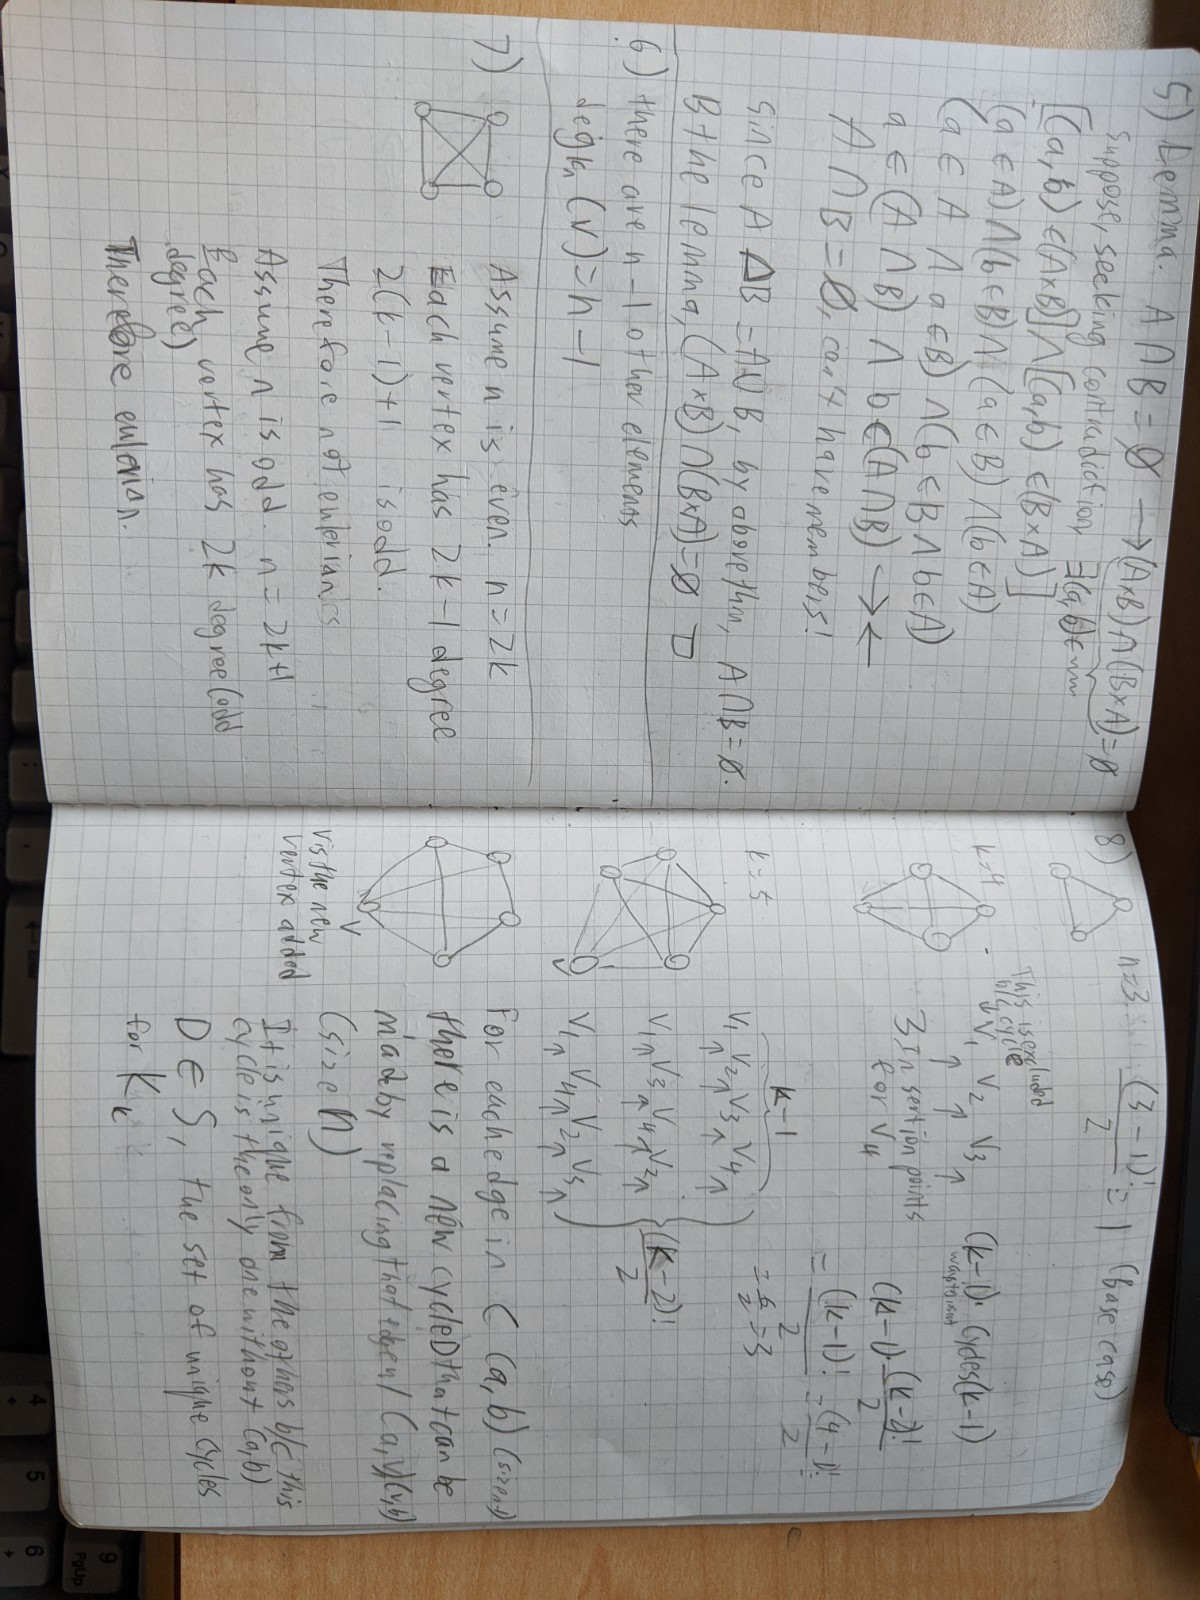
\includegraphics[angle=90, width=0.9\linewidth]{mt/2.jpg}

    \pagebreak
    
    \centering
    \thispagestyle{empty}
    \includegraphics[angle=90, width=0.9\linewidth]{mt/3.jpg}

    \pagebreak
    
    \centering
    \thispagestyle{empty}
    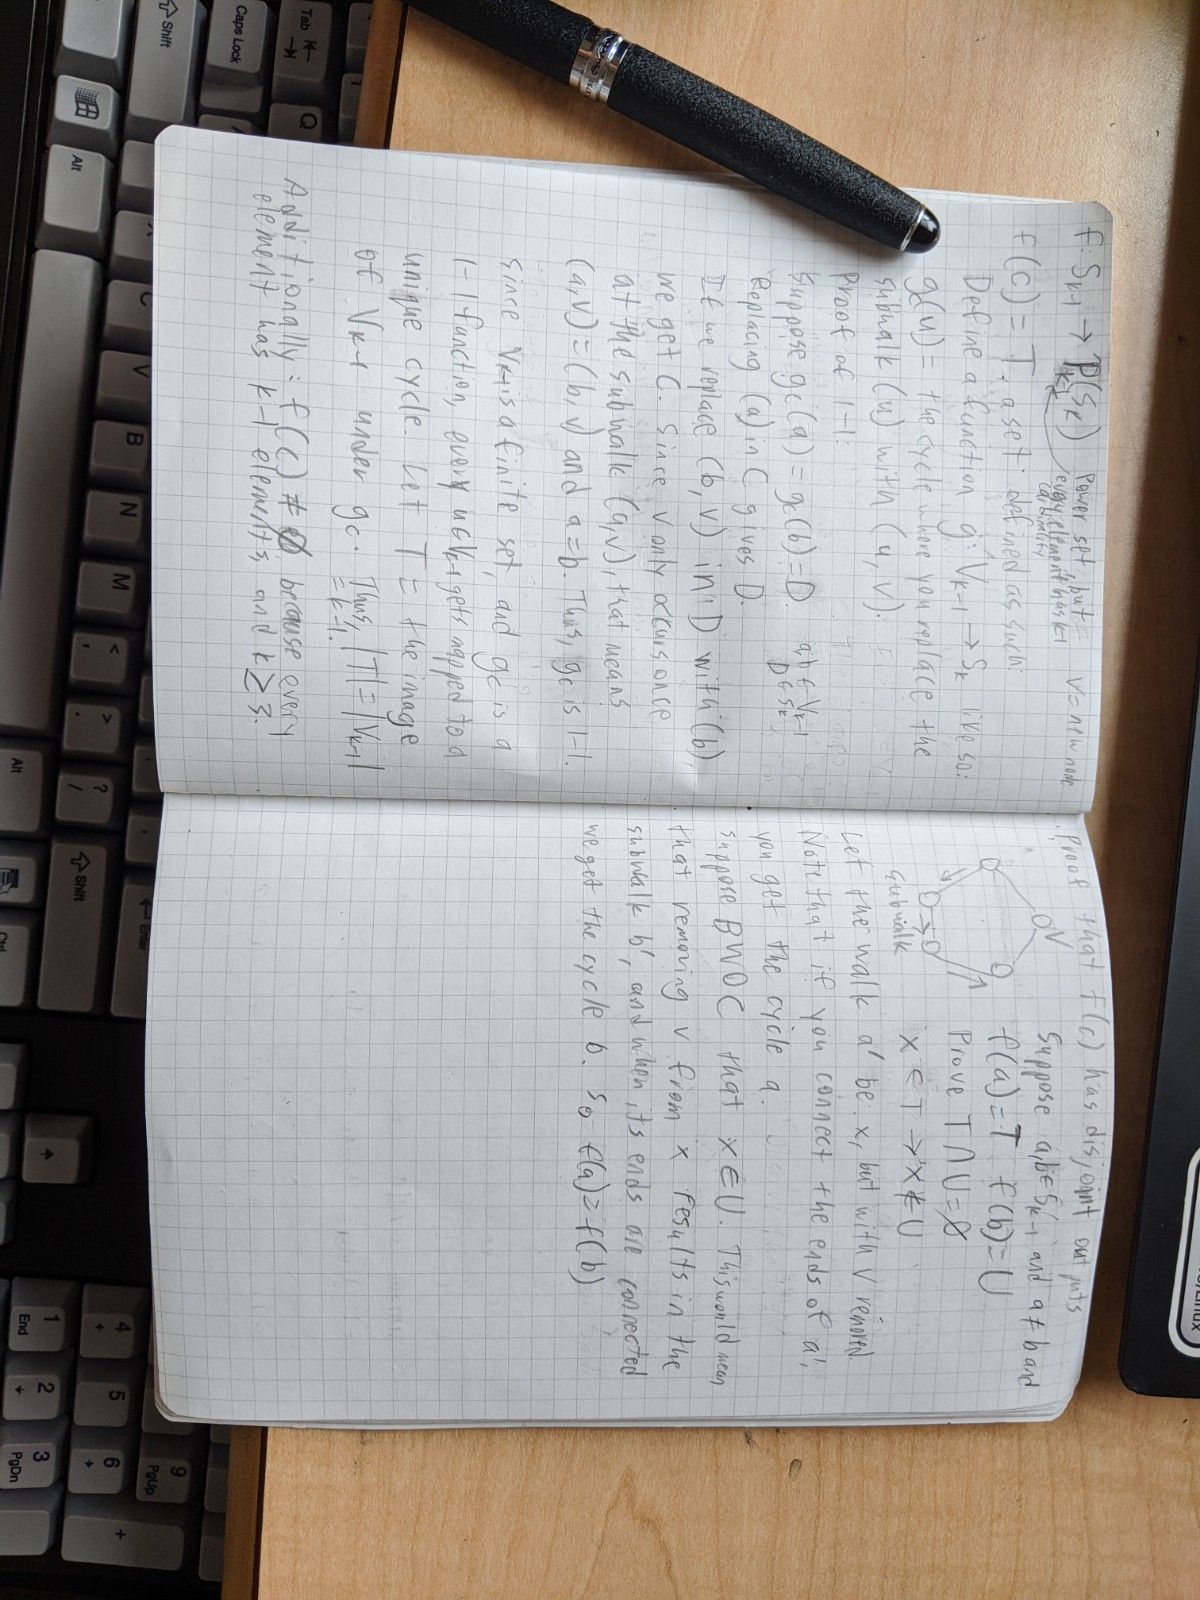
\includegraphics[angle=90, width=0.9\linewidth]{mt/4.jpg}

    \pagebreak
    
    \centering
    \thispagestyle{empty}
    \includegraphics[angle=90, width=0.9\linewidth]{mt/5.jpg}

    \pagebreak
    
    \centering
    \thispagestyle{empty}
    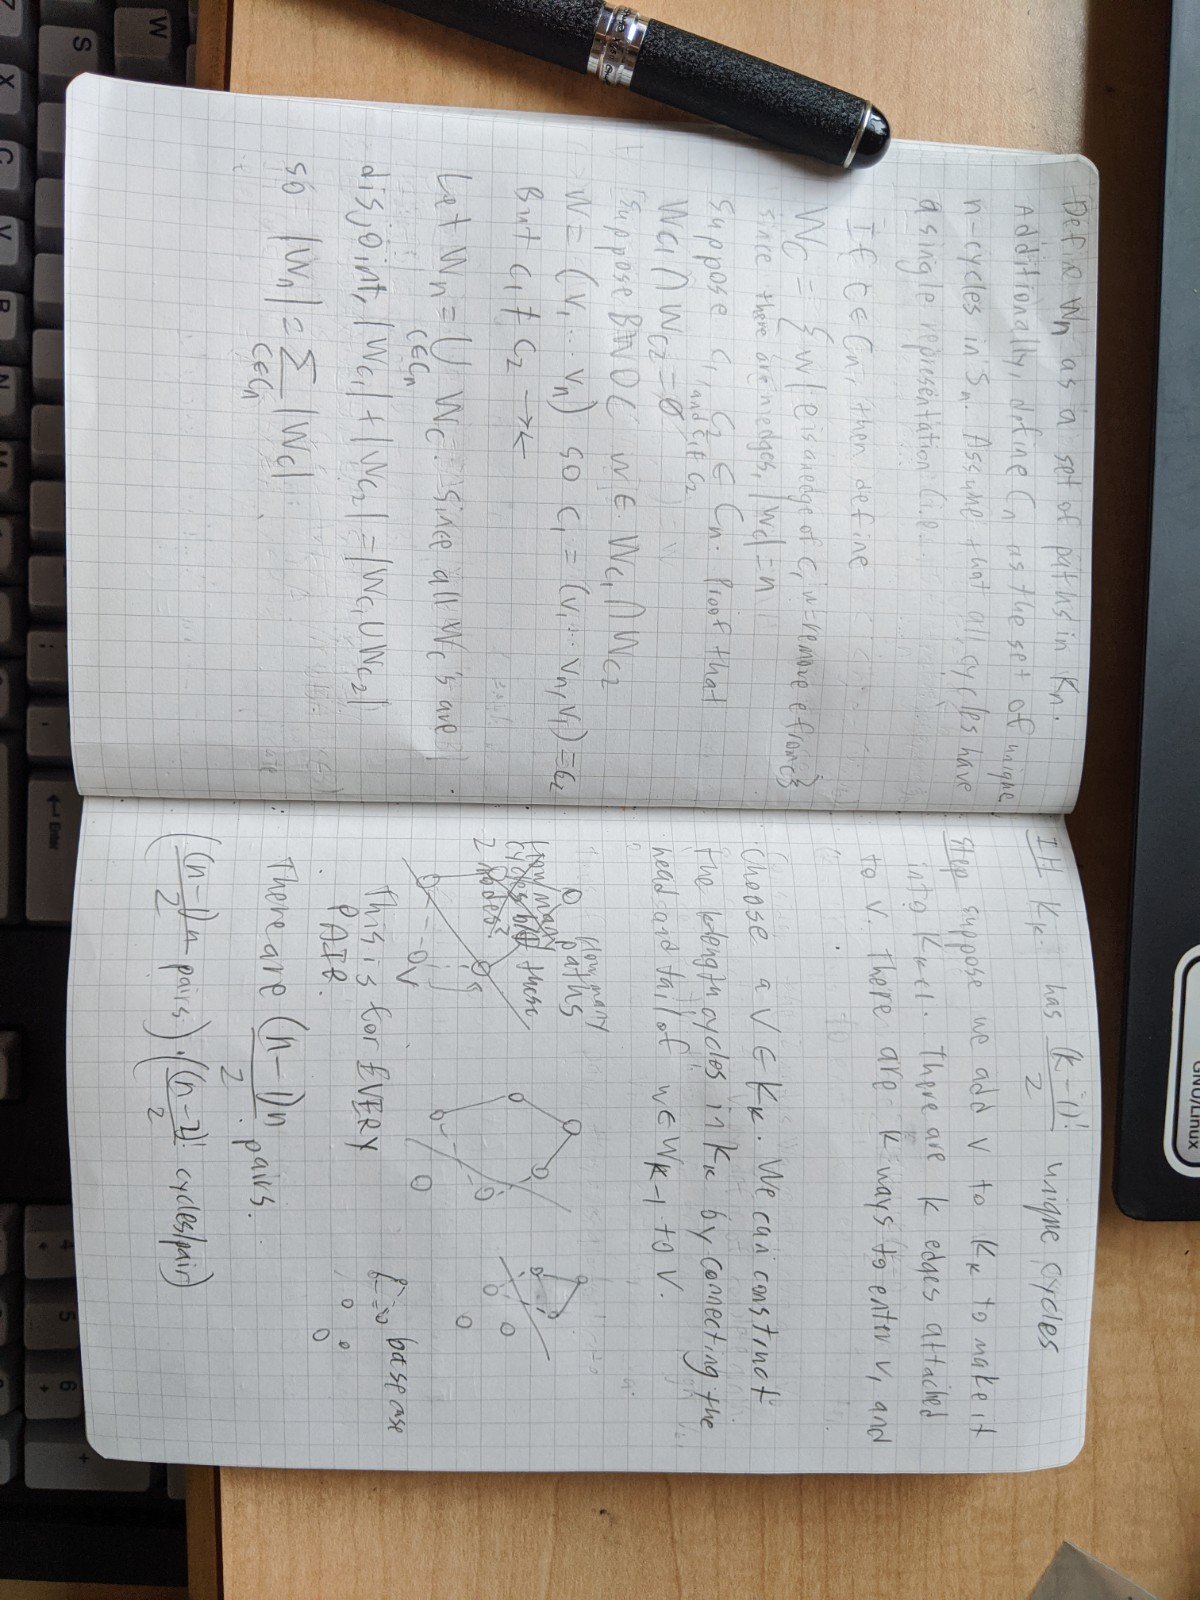
\includegraphics[angle=90, width=0.9\linewidth]{mt/6.jpg}

    \pagebreak
    
    \centering
    \thispagestyle{empty}
    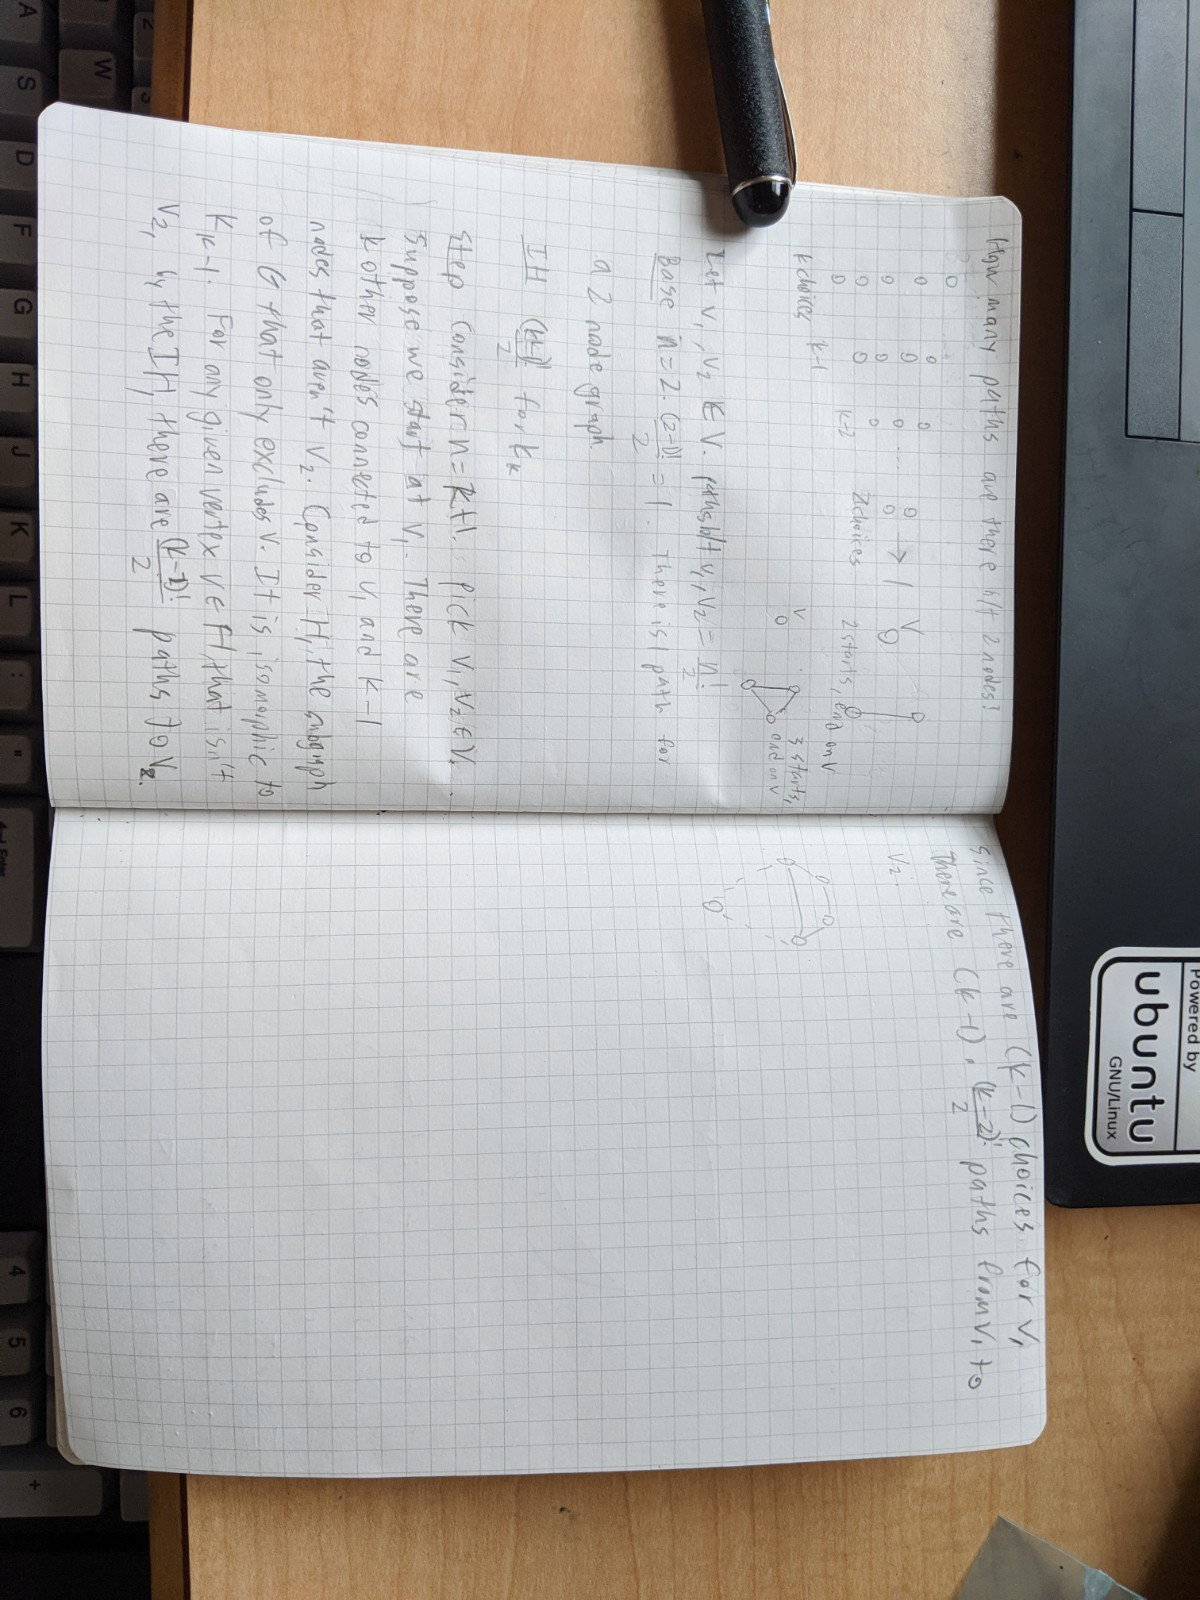
\includegraphics[angle=90, width=0.9\linewidth]{mt/7.jpg}

\end{landscape}

\restoregeometry
    
\end{document}